\subsection{Photovoltaic generator alignment} \label{sec:photovoltaic_generator_alignment}
Simply put, the alignment of a stationary PV generator -- which does not actively track the Sun throughout the day, but is installed with a fixed orientation of the normal to $A_{\mathrm{PV}}$, with respect to the cardinal directions, and a constant inclination angle $\beta$ -- depends on two basic factors.

The first factor regards the Sun's direct irradiance, which reaches its greatest daily value for clear skies at solar noon ($t_{\mathrm{S}} = 12\mathrm{h}$). This is the point in time, in which $\gamma_{\mathrm{S}}$ reaches its greatest daily value, and thus the Sun's rays have the shortest path through Earth's atmosphere to the surface. The path becomes longer, the smaller $\gamma_{\mathrm{S}}$ becomes -- regardless of whether it is before or after solar noon.\footnote{Regarding the optimal inclination angle of a PV generator for clear skies, the authors of \cite[7]{Landis:1995} write: \begin{displayquote}\textit{``For clear days, the solar irradiance is symmetrical around noon and is maximum at true solar noon, $\omega = 0$.''}\end{displayquote} The angle $\omega$ represents the solar hour angle $h_{\mathrm{S}}$.} Using the \emph{air mass} (AM) value $x$, this can be expressed as follows:
	\begin{equation} \label{eq:air_mass}
	\centering
		x = \frac{1}{\sin \gamma_{\mathrm{S}}} \text{.}
	\end{equation}
For example, for $\gamma_{\mathrm{S}} = 90^\circ$  the Sun is at its zenith. This results in $x = 1$ and therefore its rays have the shortest possible path through Earth's atmosphere to the surface. Since the spectrum of the Sun on the Earth's surface changes, depending on the length of the path of the Sun's rays, this spectrum is called AM 1. The AM 0 specturm would be outside the Earth's atmosphere which corresponds to the previously mentioned solar constant $E_{\mathrm{S}}$.  \cite{Landis:1995, Bertol:2011, Mertens:2015, Wagner:2018}. 

Besides this, the second factor regards the fact that the self-sufficent voice communication system will be in use for the entire duration of a mission. Therefore it requires electrical energy throughout the day.

Based on these findings it can be said that a stationary PV generator must be aligned in a way, so that its energy-converting area $A_{\mathrm{PV}}$ is perpendicular to the Sun's rays when it reaches its greatest daily irradiance value. This occurs when the Sun's rays have the shortest path through Earth's atmosphere. As a result, the normal to $A_{\mathrm{PV}}$ must be aligned with the incoming rays for this specific point in time, hence for $t_{\mathrm{S}} = 12\mathrm{h}$. In this case, the daily electrical energy yield of a stationary PV generator can be maximized \cite{Landis:1995, Mertens:2015, Wagner:2018}.

As mentioned in subsection \ref{sec:energy_yield}, the Sun's rays are perpendicular to the energy-converting area $A_{\mathrm{PV}}$ for $\beta = 90^\circ - \gamma_{\mathrm{S}}$. After applying this to equation (\ref{eq:sin_gamma_s}) and simplifying it with trigonometric functions, the PV generator's angle of inclinations $\beta$ at a latitude $\varphi$, with Earth's axis of rotation inclined towards the Sun with the angle $\delta$, can be derived as shown in equation (\ref{eq:beta_with_delta_and_phi}) \cite{Landis:1995, Mertens:2015, Wagner:2018}.
	\begin{equation} \label{eq:beta_with_delta_and_phi}
	\centering
		\beta = \left|\varphi - \delta\right|
	\end{equation}
The \MATLAB simulation in the appendix \ref{sec:matlab_code} showed that using the absolute value of $\beta$, it can be obtained for every installation site on Earth and for every season of the year. This is also shown by the authors of \cite{Karafil:2016}.\footnote{Nevertheless, the result of $\tan \delta \, \tan \varphi$ must be taken into account.} %However, for the equation (\ref{eq:cos_theta}) the absolute value should not be used. % CHANGE

Determining how the normal to $A_{\mathrm{PV}}$ must be oriented with respect to the cardinal directions can be accomplished by solving the equations (\ref{eq:sin_gamma_s}) and (\ref{eq:cos_alpha_s}) for $t_{\mathrm{S}} = 12\mathrm{h}$. With the help of trigonometric functions this results in:
	\begin{equation} \label{eq:gamma_s_align}
	\centering
		\gamma_{\mathrm{S}} = 90^\circ - \varphi + \delta \text{,} \quad \text{for } t_{\mathrm{S}} = 12\mathrm{h}
	\end{equation}
	\begin{equation} \label{eq:alpha_s_align}
	\centering
		\alpha_{\mathrm{S}} = \arccos \left(\frac{\sin \left(\varphi - \delta\right)}{\cos \gamma_{\mathrm{S}}}\right) \text{,} \quad \text{for } t_{\mathrm{S}} = 12\mathrm{h} \text{.}
	\end{equation}
For $\alpha_{\mathrm{S}} = 0^\circ$ the Sun is visible in the south and therefore a PV generator must be oriented in a way so that the normal to $A_{\mathrm{PV}}$ points towards the south, and for $\alpha_{\mathrm{S}} = 180^\circ$ the Sun is visible in the north and therefore the normal to $A_{\mathrm{PV}}$ must point towards the north. When the Sun is at its zenith $\alpha_{\mathrm{S}}$ cannot be solved because $\gamma_{\mathrm{S}} = 90^\circ$. In this case $\varphi = \delta$, from which $\beta = 0^\circ$ follows, and therefore the normal to $A_{\mathrm{PV}}$ must point to the Sun's zenith.

A more practical approach to this can be achieved by comparing the latitude of a PV generator's installation site to the latitude $\varphi_{\mathrm{Z}}$ in $\left(^\circ\right)$, where the Sun is at its zenith for $t_{\mathrm{S}} = 12\mathrm{h}$, using a GPS device. Figure \ref{fig:crucial_latitudes} compares the three different cases of the Sun's location in the sky, depending on the installation site of a PV generator, in which $\varphi_{\mathrm{S}}$ in $\left(^\circ\right)$ is an installation site to the south and $\varphi_{\mathrm{N}}$ in $\left(^\circ\right)$ to the north of $\varphi_{\mathrm{Z}}$.

\begin{figure}[h!]
	\centering
		\begin{subfigure}[b]{0.3\linewidth}
			

\tikzset{every picture/.style={line width=0.75pt}} %set default line width to 0.75pt        

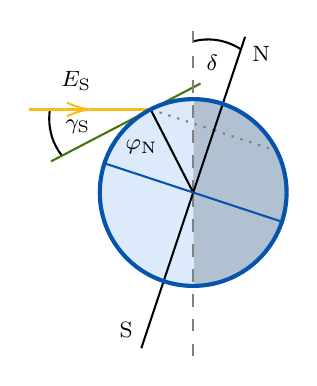
\begin{tikzpicture}[x=0.75pt,y=0.75pt,yscale=-1,xscale=1]
%uncomment if require: \path (0,201); %set diagram left start at 0, and has height of 201

%Shape: Pie [id:dp4750642586964353] 
\draw  [color={rgb, 255:red, 0; green, 0; blue, 0 }  ,draw opacity=0 ][fill={rgb, 255:red, 0; green, 0; blue, 0 }  ,fill opacity=0.45 ] (93.03,60.03) .. controls (117.81,60.3) and (137.85,80.25) .. (137.93,104.89) .. controls (138.02,129.63) and (117.94,149.78) .. (93.03,150.05) -- (92.52,105.04) -- cycle ;
%Shape: Circle [id:dp9006978183202985] 
\draw  [color={rgb, 255:red, 7; green, 84; blue, 173 }  ,draw opacity=1 ][fill={rgb, 255:red, 200; green, 222; blue, 248 }  ,fill opacity=0.64 ][line width=0.75]  (47.52,105.04) .. controls (47.52,80.19) and (67.67,60.04) .. (92.52,60.04) .. controls (117.38,60.04) and (137.52,80.19) .. (137.52,105.04) .. controls (137.52,129.89) and (117.38,150.04) .. (92.52,150.04) .. controls (67.67,150.04) and (47.52,129.89) .. (47.52,105.04) -- cycle ;
%Straight Lines [id:da06282467353758259] 
\draw [color={rgb, 255:red, 65; green, 117; blue, 5 }  ,draw opacity=1 ]   (96.02,52.54) -- (72.02,65.04) ;
%Shape: Arc [id:dp49173933797962777] 
\draw  [draw opacity=0] (29.42,87.46) .. controls (28.29,86.06) and (27.29,84.54) .. (26.43,82.91) .. controls (23.51,77.38) and (22.61,71.21) .. (23.45,65.01) -- (66.02,62.04) -- cycle ; \draw   (29.42,87.46) .. controls (28.29,86.06) and (27.29,84.54) .. (26.43,82.91) .. controls (23.51,77.38) and (22.61,71.21) .. (23.45,65.01) ;
%Straight Lines [id:da6550544250175496] 
\draw [color={rgb, 255:red, 65; green, 117; blue, 5 }  ,draw opacity=1 ]   (24.02,90.04) -- (72.02,65.04) ;
%Shape: Arc [id:dp963370582460114] 
\draw  [draw opacity=0] (92.23,32.3) .. controls (94.76,31.6) and (97.38,31.25) .. (100.07,31.29) .. controls (105.67,31.35) and (110.94,33.08) .. (115.6,36.08) -- (99.52,76.04) -- cycle ; \draw   (92.23,32.3) .. controls (94.76,31.6) and (97.38,31.25) .. (100.07,31.29) .. controls (105.67,31.35) and (110.94,33.08) .. (115.6,36.08) ;
%Straight Lines [id:da058893605247020586] 
\draw [color={rgb, 255:red, 128; green, 128; blue, 128 }  ,draw opacity=1 ] [dash pattern={on 4.5pt off 4.5pt}]  (92.52,183.96) -- (92.52,105.04) ;
%Straight Lines [id:da5478983474017609] 
\draw [color={rgb, 255:red, 128; green, 128; blue, 128 }  ,draw opacity=1 ] [dash pattern={on 4.5pt off 4.5pt}]  (92.52,105.04) -- (92.52,26.12) ;
%Straight Lines [id:da4780085054484584] 
\draw [line width=0.75]    (72.02,65.04) -- (92.52,105.04) ;
%Straight Lines [id:da5291514924825897] 
\draw [color={rgb, 255:red, 128; green, 128; blue, 128 }  ,draw opacity=1 ] [dash pattern={on 0.84pt off 2.51pt}]  (102.52,75.04) -- (133.02,85.04) ;
%Straight Lines [id:da4294056374442512] 
\draw [color={rgb, 255:red, 128; green, 128; blue, 128 }  ,draw opacity=1 ] [dash pattern={on 0.84pt off 2.51pt}]  (72.02,65.04) -- (102.52,75.04) ;
%Straight Lines [id:da35119327320040794] 
\draw    (92.52,105.04) -- (67.52,180.04) ;
%Straight Lines [id:da9687000233514724] 
\draw    (117.52,30.04) -- (92.52,105.04) ;
%Straight Lines [id:da8818616046820387] 
\draw [color={rgb, 255:red, 7; green, 84; blue, 173 }  ,draw opacity=1 ]   (50.02,91.04) -- (92.52,105.04) ;
%Straight Lines [id:da4795343191360564] 
\draw [color={rgb, 255:red, 7; green, 84; blue, 173 }  ,draw opacity=1 ]   (92.52,105.04) -- (135.02,119.04) ;
%Straight Lines [id:da6396043564859444] 
\draw [color={rgb, 255:red, 248; green, 189; blue, 28 }  ,draw opacity=1 ]   (42.65,65.04) -- (72.02,65.04) ;
%Straight Lines [id:da3150442288480175] 
\draw [color={rgb, 255:red, 248; green, 189; blue, 28 }  ,draw opacity=1 ]   (13.27,65.04) -- (40.65,65.04) ;
\draw [shift={(42.65,65.04)}, rotate = 180] [color={rgb, 255:red, 248; green, 189; blue, 28 }  ,draw opacity=1 ][line width=0.75]    (10.93,-3.29) .. controls (6.95,-1.4) and (3.31,-0.3) .. (0,0) .. controls (3.31,0.3) and (6.95,1.4) .. (10.93,3.29)   ;
%Shape: Circle [id:dp4877206756511603] 
\draw  [color={rgb, 255:red, 7; green, 84; blue, 173 }  ,draw opacity=1 ][fill={rgb, 255:red, 200; green, 222; blue, 248 }  ,fill opacity=0 ][line width=1.5]  (47.52,105.04) .. controls (47.52,80.19) and (67.67,60.04) .. (92.52,60.04) .. controls (117.38,60.04) and (137.52,80.19) .. (137.52,105.04) .. controls (137.52,129.89) and (117.38,150.04) .. (92.52,150.04) .. controls (67.67,150.04) and (47.52,129.89) .. (47.52,105.04) -- cycle ;

% Text Node
\draw (58.52,78.4) node [anchor=north west][inner sep=0.75pt]  [font=\footnotesize]  {$\varphi _{\mathrm{N}}$};
% Text Node
\draw (97.52,37.44) node [anchor=north west][inner sep=0.75pt]  [font=\footnotesize]  {$\delta $};
% Text Node
\draw (29.52,68.44) node [anchor=north west][inner sep=0.75pt]  [font=\footnotesize]  {$\gamma _{\mathrm{S}}$};
% Text Node
\draw (27.52,45.4) node [anchor=north west][inner sep=0.75pt]  [font=\footnotesize]  {$E_{\mathrm{S}}$};
% Text Node
\draw (119.52,33.04) node [anchor=north west][inner sep=0.75pt]  [font=\footnotesize] [align=left] {N};
% Text Node
\draw (55.52,166.04) node [anchor=north west][inner sep=0.75pt]  [font=\footnotesize] [align=left] {S};


\end{tikzpicture}

			\caption{Northern latitude.}
		\end{subfigure}
		\begin{subfigure}[b]{0.3\linewidth}
			

\tikzset{every picture/.style={line width=0.75pt}} %set default line width to 0.75pt        

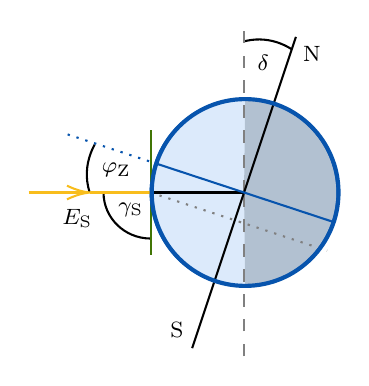
\begin{tikzpicture}[x=0.75pt,y=0.75pt,yscale=-1,xscale=1]
%uncomment if require: \path (0,181); %set diagram left start at 0, and has height of 181

%Shape: Arc [id:dp20953347708018688] 
\draw  [draw opacity=0] (69.43,111.09) .. controls (69.33,111.09) and (69.24,111.09) .. (69.15,111.09) .. controls (56.73,110.92) and (46.77,101.07) .. (46.73,89) -- (69.44,88.92) -- cycle ; \draw   (69.43,111.09) .. controls (69.33,111.09) and (69.24,111.09) .. (69.15,111.09) .. controls (56.73,110.92) and (46.77,101.07) .. (46.73,89) ;
%Shape: Arc [id:dp16591242877449974] 
\draw  [draw opacity=0] (40.06,88.92) .. controls (39.51,87.21) and (39.11,85.44) .. (38.89,83.61) .. controls (38.13,77.4) and (39.47,71.31) .. (42.46,65.81) -- (83.31,78.18) -- cycle ; \draw   (40.06,88.92) .. controls (39.51,87.21) and (39.11,85.44) .. (38.89,83.61) .. controls (38.13,77.4) and (39.47,71.31) .. (42.46,65.81) ;
%Straight Lines [id:da6013522376382066] 
\draw [color={rgb, 255:red, 65; green, 117; blue, 5 }  ,draw opacity=1 ]   (69.44,118.92) -- (69.44,88.92) ;
%Shape: Pie [id:dp028486029029515914] 
\draw  [color={rgb, 255:red, 0; green, 0; blue, 0 }  ,draw opacity=0 ][fill={rgb, 255:red, 0; green, 0; blue, 0 }  ,fill opacity=0.45 ] (114.95,43.91) .. controls (139.73,44.18) and (159.77,64.13) .. (159.85,88.77) .. controls (159.93,113.51) and (139.86,133.66) .. (114.94,133.93) -- (114.44,88.92) -- cycle ;
%Shape: Circle [id:dp7286185522053927] 
\draw  [color={rgb, 255:red, 7; green, 84; blue, 173 }  ,draw opacity=1 ][fill={rgb, 255:red, 200; green, 222; blue, 248 }  ,fill opacity=0.64 ][line width=0.75]  (69.44,88.92) .. controls (69.44,64.07) and (89.59,43.92) .. (114.44,43.92) .. controls (139.29,43.92) and (159.44,64.07) .. (159.44,88.92) .. controls (159.44,113.77) and (139.29,133.92) .. (114.44,133.92) .. controls (89.59,133.92) and (69.44,113.77) .. (69.44,88.92) -- cycle ;
%Shape: Arc [id:dp17913789171454497] 
\draw  [draw opacity=0] (114.15,16.18) .. controls (116.67,15.49) and (119.3,15.14) .. (121.99,15.17) .. controls (127.58,15.24) and (132.85,16.96) .. (137.52,19.97) -- (121.44,59.92) -- cycle ; \draw   (114.15,16.18) .. controls (116.67,15.49) and (119.3,15.14) .. (121.99,15.17) .. controls (127.58,15.24) and (132.85,16.96) .. (137.52,19.97) ;
%Straight Lines [id:da9967059081670446] 
\draw [color={rgb, 255:red, 128; green, 128; blue, 128 }  ,draw opacity=1 ] [dash pattern={on 4.5pt off 4.5pt}]  (114.44,167.84) -- (114.44,88.92) ;
%Straight Lines [id:da71597890822506] 
\draw [color={rgb, 255:red, 128; green, 128; blue, 128 }  ,draw opacity=1 ] [dash pattern={on 4.5pt off 4.5pt}]  (114.44,88.92) -- (114.44,10) ;
%Straight Lines [id:da4137878061890663] 
\draw [color={rgb, 255:red, 128; green, 128; blue, 128 }  ,draw opacity=1 ] [dash pattern={on 0.84pt off 2.51pt}]  (69.44,88.92) -- (111.94,102.92) ;
%Straight Lines [id:da3390187694217488] 
\draw [color={rgb, 255:red, 128; green, 128; blue, 128 }  ,draw opacity=1 ] [dash pattern={on 0.84pt off 2.51pt}]  (111.94,102.92) -- (154.44,116.92) ;
%Straight Lines [id:da5052190602488993] 
\draw    (114.44,88.92) -- (89.44,163.92) ;
%Straight Lines [id:da6983846735857875] 
\draw    (139.44,13.92) -- (114.44,88.92) ;
%Straight Lines [id:da5175201690882127] 
\draw    (69.44,88.92) -- (114.44,88.92) ;
%Straight Lines [id:da23163800871480023] 
\draw [color={rgb, 255:red, 65; green, 117; blue, 5 }  ,draw opacity=1 ]   (69.44,88.92) -- (69.44,58.92) ;
%Straight Lines [id:da47404926603772557] 
\draw [color={rgb, 255:red, 7; green, 84; blue, 173 }  ,draw opacity=1 ] [dash pattern={on 0.84pt off 2.51pt}]  (29.44,60.92) -- (71.94,74.92) ;
%Straight Lines [id:da6548182479176137] 
\draw [color={rgb, 255:red, 248; green, 189; blue, 28 }  ,draw opacity=1 ]   (10.69,88.92) -- (38.06,88.92) ;
\draw [shift={(40.06,88.92)}, rotate = 180] [color={rgb, 255:red, 248; green, 189; blue, 28 }  ,draw opacity=1 ][line width=0.75]    (10.93,-3.29) .. controls (6.95,-1.4) and (3.31,-0.3) .. (0,0) .. controls (3.31,0.3) and (6.95,1.4) .. (10.93,3.29)   ;
%Straight Lines [id:da7518207882403078] 
\draw [color={rgb, 255:red, 248; green, 189; blue, 28 }  ,draw opacity=1 ]   (40.06,88.92) -- (69.44,88.92) ;
%Shape: Circle [id:dp4417291051670942] 
\draw  [color={rgb, 255:red, 7; green, 84; blue, 173 }  ,draw opacity=1 ][fill={rgb, 255:red, 200; green, 222; blue, 248 }  ,fill opacity=0 ][line width=1.5]  (69.95,88.91) .. controls (69.95,64.06) and (90.1,43.91) .. (114.95,43.91) .. controls (139.8,43.91) and (159.95,64.06) .. (159.95,88.91) .. controls (159.95,113.77) and (139.8,133.91) .. (114.95,133.91) .. controls (90.1,133.91) and (69.95,113.77) .. (69.95,88.91) -- cycle ;
%Straight Lines [id:da09584357360735729] 
\draw [color={rgb, 255:red, 7; green, 84; blue, 173 }  ,draw opacity=1 ]   (71.94,74.92) -- (114.44,88.92) ;
%Straight Lines [id:da1322107965109387] 
\draw [color={rgb, 255:red, 7; green, 84; blue, 173 }  ,draw opacity=1 ]   (114.44,88.92) -- (156.94,102.92) ;

% Text Node
\draw (44.44,73.32) node [anchor=north west][inner sep=0.75pt]  [font=\footnotesize]  {$\varphi _{\mathrm{Z}}$};
% Text Node
\draw (119.44,21.32) node [anchor=north west][inner sep=0.75pt]  [font=\footnotesize]  {$\delta $};
% Text Node
\draw (25.44,95.4) node [anchor=north west][inner sep=0.75pt]  [font=\footnotesize]  {$E_{\mathrm{S}}$};
% Text Node
\draw (141.44,16.92) node [anchor=north west][inner sep=0.75pt]  [font=\footnotesize] [align=left] {N};
% Text Node
\draw (77.44,149.92) node [anchor=north west][inner sep=0.75pt]  [font=\footnotesize] [align=left] {S};
% Text Node
\draw (52.44,92.32) node [anchor=north west][inner sep=0.75pt]  [font=\footnotesize]  {$\gamma _{\mathrm{S}}$};


\end{tikzpicture}

			\caption{Sun is at its zenith.}
		\end{subfigure}
		\begin{subfigure}[b]{0.3\linewidth}
			

\tikzset{every picture/.style={line width=0.75pt}} %set default line width to 0.75pt        

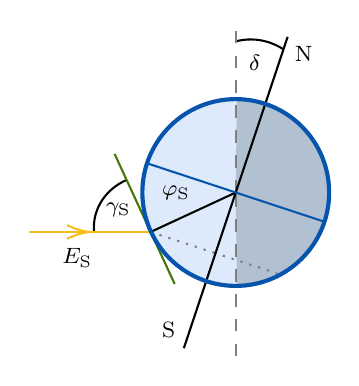
\begin{tikzpicture}[x=0.75pt,y=0.75pt,yscale=-1,xscale=1]
%uncomment if require: \path (0,181); %set diagram left start at 0, and has height of 181

%Shape: Arc [id:dp1509931683753729] 
\draw  [draw opacity=0] (41.51,107.98) .. controls (41.44,107.22) and (41.4,106.45) .. (41.4,105.68) .. controls (41.4,95.62) and (47.84,86.94) .. (57.17,82.86) -- (69.17,105.68) -- cycle ; \draw   (41.51,107.98) .. controls (41.44,107.22) and (41.4,106.45) .. (41.4,105.68) .. controls (41.4,95.62) and (47.84,86.94) .. (57.17,82.86) ;
%Shape: Pie [id:dp008234319355738817] 
\draw  [color={rgb, 255:red, 0; green, 0; blue, 0 }  ,draw opacity=0 ][fill={rgb, 255:red, 0; green, 0; blue, 0 }  ,fill opacity=0.45 ] (110.26,43.91) .. controls (135.04,44.18) and (155.08,64.13) .. (155.16,88.77) .. controls (155.24,113.51) and (135.17,133.66) .. (110.25,133.93) -- (109.75,88.92) -- cycle ;
%Shape: Circle [id:dp3321431212746069] 
\draw  [color={rgb, 255:red, 7; green, 84; blue, 173 }  ,draw opacity=1 ][fill={rgb, 255:red, 200; green, 222; blue, 248 }  ,fill opacity=0.64 ][line width=0.75]  (64.75,88.92) .. controls (64.75,64.07) and (84.9,43.92) .. (109.75,43.92) .. controls (134.6,43.92) and (154.75,64.07) .. (154.75,88.92) .. controls (154.75,113.77) and (134.6,133.92) .. (109.75,133.92) .. controls (84.9,133.92) and (64.75,113.77) .. (64.75,88.92) -- cycle ;
%Straight Lines [id:da8319048303736489] 
\draw [color={rgb, 255:red, 65; green, 117; blue, 5 }  ,draw opacity=1 ]   (57.17,82.86) -- (68.75,107.92) ;
%Shape: Arc [id:dp7416942399851174] 
\draw  [draw opacity=0] (109.46,16.18) .. controls (111.99,15.49) and (114.61,15.14) .. (117.3,15.17) .. controls (122.89,15.24) and (128.16,16.96) .. (132.83,19.97) -- (116.75,59.92) -- cycle ; \draw   (109.46,16.18) .. controls (111.99,15.49) and (114.61,15.14) .. (117.3,15.17) .. controls (122.89,15.24) and (128.16,16.96) .. (132.83,19.97) ;
%Straight Lines [id:da23785833539369183] 
\draw [color={rgb, 255:red, 128; green, 128; blue, 128 }  ,draw opacity=1 ] [dash pattern={on 4.5pt off 4.5pt}]  (109.75,167.84) -- (109.75,88.92) ;
%Straight Lines [id:da06972248148475568] 
\draw [color={rgb, 255:red, 128; green, 128; blue, 128 }  ,draw opacity=1 ] [dash pattern={on 4.5pt off 4.5pt}]  (109.75,88.92) -- (109.75,10) ;
%Straight Lines [id:da8960602024330377] 
\draw [line width=0.75]    (68.75,107.92) -- (109.75,88.92) ;
%Straight Lines [id:da5098060920131091] 
\draw [color={rgb, 255:red, 128; green, 128; blue, 128 }  ,draw opacity=1 ] [dash pattern={on 0.84pt off 2.51pt}]  (99.25,117.92) -- (129.75,127.92) ;
%Straight Lines [id:da8906380552334501] 
\draw [color={rgb, 255:red, 128; green, 128; blue, 128 }  ,draw opacity=1 ] [dash pattern={on 0.84pt off 2.51pt}]  (68.75,107.92) -- (99.25,117.92) ;
%Straight Lines [id:da14349690184184327] 
\draw    (109.75,88.92) -- (84.75,163.92) ;
%Straight Lines [id:da024036142327008347] 
\draw    (134.75,13.92) -- (109.75,88.92) ;
%Straight Lines [id:da21245027564913532] 
\draw [color={rgb, 255:red, 7; green, 84; blue, 173 }  ,draw opacity=1 ]   (67.25,74.92) -- (109.75,88.92) ;
%Straight Lines [id:da7748765899346521] 
\draw [color={rgb, 255:red, 7; green, 84; blue, 173 }  ,draw opacity=1 ]   (109.75,88.92) -- (152.25,102.92) ;
%Straight Lines [id:da645165483038932] 
\draw [color={rgb, 255:red, 65; green, 117; blue, 5 }  ,draw opacity=1 ]   (68.75,107.92) -- (80.33,132.98) ;
%Straight Lines [id:da01702325380082992] 
\draw [color={rgb, 255:red, 65; green, 117; blue, 5 }  ,draw opacity=1 ]   (57.17,82.86) -- (51.38,70.33) ;
%Straight Lines [id:da7674893611261671] 
\draw [color={rgb, 255:red, 248; green, 189; blue, 28 }  ,draw opacity=1 ]   (39.38,107.92) -- (68.75,107.92) ;
%Straight Lines [id:da5473156330354862] 
\draw [color={rgb, 255:red, 248; green, 189; blue, 28 }  ,draw opacity=1 ]   (10,107.92) -- (37.38,107.92) ;
\draw [shift={(39.38,107.92)}, rotate = 180] [color={rgb, 255:red, 248; green, 189; blue, 28 }  ,draw opacity=1 ][line width=0.75]    (10.93,-3.29) .. controls (6.95,-1.4) and (3.31,-0.3) .. (0,0) .. controls (3.31,0.3) and (6.95,1.4) .. (10.93,3.29)   ;
%Shape: Circle [id:dp46167221588038543] 
\draw  [color={rgb, 255:red, 7; green, 84; blue, 173 }  ,draw opacity=1 ][fill={rgb, 255:red, 200; green, 222; blue, 248 }  ,fill opacity=0 ][line width=1.5]  (64.75,88.92) .. controls (64.75,64.07) and (84.9,43.92) .. (109.75,43.92) .. controls (134.6,43.92) and (154.75,64.07) .. (154.75,88.92) .. controls (154.75,113.77) and (134.6,133.92) .. (109.75,133.92) .. controls (84.9,133.92) and (64.75,113.77) .. (64.75,88.92) -- cycle ;

% Text Node
\draw (72.75,84.32) node [anchor=north west][inner sep=0.75pt]  [font=\footnotesize]  {$\varphi _{\mathrm{S}}$};
% Text Node
\draw (114.75,21.32) node [anchor=north west][inner sep=0.75pt]  [font=\footnotesize]  {$\delta $};
% Text Node
\draw (45.75,92.32) node [anchor=north west][inner sep=0.75pt]  [font=\footnotesize]  {$\gamma _{\mathrm{S}}$};
% Text Node
\draw (24.75,114.32) node [anchor=north west][inner sep=0.75pt]  [font=\footnotesize]  {$E_{\mathrm{S}}$};
% Text Node
\draw (136.75,16.92) node [anchor=north west][inner sep=0.75pt]  [font=\footnotesize] [align=left] {N};
% Text Node
\draw (72.75,149.92) node [anchor=north west][inner sep=0.75pt]  [font=\footnotesize] [align=left] {S};


\end{tikzpicture}

			\caption{Southern latitude.}
		\end{subfigure}
	\caption{Illustration of the latitude $\varphi_{\mathrm{Z}}$ on Earth at which the Sun is at its zenith for $t_{\mathrm{S}} = 12\mathrm{h}$. By comparing the latitude of the installation site of a photovoltaic generator it can be determined how it must be aligned, so that the electrical energy yield can be maximized.}
	\label{fig:crucial_latitudes}
\end{figure}

Inserting $\gamma_{\mathrm{S}} = 90^\circ$ and $t_{\mathrm{S}} = 12\mathrm{h}$ into equation (\ref{eq:sin_gamma_s}), the latitude $\varphi_{\mathrm{Z}}$ can be determined -- after applying trigonometric functions -- to:
	\begin{equation} \label{eq:phi_z}
	\centering
		\varphi_{\mathrm{Z}} = \delta \text{.}
	\end{equation}
If a PV generator is installed at a latitude south of $\varphi_{\mathrm{Z}}$, the normal to $A_{\mathrm{PV}}$ must point towards the north, and if it is installed north of $\varphi_{\mathrm{Z}}$, the normal to $A_{\mathrm{PV}}$ must point towards the south. In case the PV generator is installed at the latitude $\varphi_{\mathrm{Z}}$, then $\beta = \varphi_{\mathrm{Z}} - \delta = 0^\circ$ applies, which means that the normal to $A_{\mathrm{PV}}$ points to the Sun's zenith. The normal to $A_{\mathrm{PV}}$ can be aligned using a simple compass.
